\documentclass{article}
% pre\'ambulo

\usepackage{lmodern}
\usepackage[T1]{fontenc}
\usepackage[spanish,activeacute]{babel}
\usepackage{mathtools}
\usepackage{graphicx}
\usepackage{listings}
\usepackage{tabu}
\usepackage{hyperref}
\usepackage[utf8]{inputenc}
\usepackage{multicol}
\usepackage{amsmath}
\usepackage{amssymb}
\usepackage{enumerate}
\usepackage{amsthm}
\usepackage{wrapfig}
\usepackage{esvect}
\usepackage{subcaption}
%\usepackage{wasysym}
\usepackage{mathabx}
\usepackage{adjustbox}

\spanishdecimal{.}


\newenvironment{myfont}{\fontfamily{pnc}\selectfont}{\par}



% Default fixed font does not support bold face
\DeclareFixedFont{\ttb}{T1}{txtt}{bx}{n}{8} % for bold
\DeclareFixedFont{\ttm}{T1}{txtt}{m}{n}{8}  % for normal

% Custom colors
\usepackage[usenames,dvipsnames]{color}
\definecolor{deepblue}{rgb}{0,0,0.5}
\definecolor{deepred}{rgb}{0.6,0,0}
\definecolor{deepgreen}{rgb}{0,0.5,0}

% Python style for highlighting
\newcommand\pythonstyle{\lstset{
language=Python,
basicstyle=\ttm,
otherkeywords={self},             % Add keywords here
keywordstyle=\ttb\color{deepblue},
emph={MyClass,__init__},          % Custom highlighting
emphstyle=\ttb\color{deepred},    % Custom highlighting style
stringstyle=\color{deepgreen},
frame=tb,                         % Any extra options here
showstringspaces=false            % 
}}


% Python environment
\lstnewenvironment{python}[1][]
{
\pythonstyle
\lstset{#1}
}
{}

% Python for external files
\newcommand\pythonexternal[2][]{{
\pythonstyle
\lstinputlisting[#1]{#2}}}

% Python for inline
\newcommand\pythoninline[1]{{\pythonstyle\lstinline!#1!}}

\usepackage{amsmath} % or simply amstext
\newcommand{\angstrom}{\text{\normalfont\AA}}
\newcommand*{\everymodeprime}{\ensuremath{\prime}}

\title{Tarea 1}
\author{Francisco Felipe Carrasco Varela}

\usepackage{vmargin}

\setpapersize{A4}
\setmargins{1.82cm}       % margen izquierdo
{1.3cm}                        % margen superior
{17.5cm}                      % anchura del texto
{23.42cm}                    % altura del texto
{10pt}                           % altura de los encabezados
{1cm}                           % espacio entre el texto y los encabezados
{0pt}                             % altura del pie de página
{2cm}                           % espacio entre el texto y el pie de página

\usepackage{array,booktabs,tabularx,caption, ragged2e}
\newcolumntype{C}{>{\centering\arraybackslash}X}

\begin{document}
\begin{minipage}{2.3cm}

\includegraphics[width=2cm]{../logo_byn.png}
\vspace{0.5cm}
\end{minipage}
\begin{minipage}{\linewidth}
\textsc{\raggedright \footnotesize
Pontificia Universidad Católica de Chile \\
Facultad de Física -- Instituto de Astrof'isica \\
Astronom'ia -- AST0111 \\
Primer Semestre 2020}
\end{minipage}
\begin{center}
{\LARGE \textbf{Ayudant'ia 5 -- Soluci'on}}

\vspace{3mm}

Profesora: Viviana Guzm'an

Ayudantes: Camila Aravena Gonz'alez (\texttt{cfaravena1$@$uc.cl}) -- Francisco Carrasco Varela (\texttt{ffcarrasco$@$uc.cl})

\end{center}
\begin{center}
\noindent\rule{12cm}{0.4pt}
\end{center}

\begin{center}
\begin{tabularx}{\linewidth}{*{6}{C}} \toprule
Planeta & Masa ($\rm kg$) & Volumen ($\rm km^3$) & Densidad media ($\rm \frac{gr}{cm^3}$) & {\small Per'iodo Rotaci'on} ({\small D'ias terrestres}) & Per'iodo Orbital ({\small A'nos terrestres}) \\\midrule
Mercurio ($\Mercury$) &  $3.3 \times 10^{23}$ & $6.08 \times 10^{10}$ & $5.42$ & $58.6$ & $0.24$\\
Venus ($\Venus$) & $4.86 \times 10^{24}$ & $9.28 \times 10^{11}$ & $5.24$ & $243$ & $0.61$\\
Tierra ($\Earth$) & $5.97 \times 10^{24}$ & $1.08 \times 10^{12}$ & $5.51$ & $1$ & $1.00$\\
Marte ($\Mars$) & $6.4 \times 10^{23}$ & $1.63 \times 10^{11}$& $3.93$& $1.03$ & $1.88$\\
J'upiter ($\Jupiter$) & $1.89 \times 10^{27}$ & $1.43 \times 10^{15}$ & $1.33$& $0.41$ & $11.86$\\
Saturno ($\Saturn$) & $5.68 \times 10^{26}$ & $8.27 \times 10^{14}$ & $0.68$ & $0.42$ & $29.46$\\
Urano ($\Uranus$) & $8.68 \times 10^{25}$ & $6.83 \times 10^{13}$ & $1.27$ & $0.71$ & $84.01$\\ 
Neptuno ($\Neptune$) & $1.02 \times 10^{26}$ & $6.25 \times 10^{13}$& $1.63$ & $0.67$ & $164.79$\\\bottomrule
\hline
\end{tabularx}
\captionof{table}{Algunos datos sobre los planetas del Sistema Solar.}   \label{tabla_planetas}
\end{center}

\textbf{Problema 1. Caracter'isticas generales de planetas gaseosos (jovianos)}

\vspace{3mm}

\begin{enumerate}[a)] 

\begin{myfont}\item ¿Cu'ales son los planetas gaseosos? \end{myfont}

\emph{Soluci'on:}

\begin{multicols}{2}

\begin{itemize}
\item J'upiter
\item Saturno
\item Urano
\item Neptuno
\end{itemize}
\end{multicols}



\begin{myfont} \item ¿Cu'ales son los m'as grandes de ellos? \end{myfont}

\emph{Soluci'on:}


Tanto en masa como en volumen, los dos planetas m'as grandes -tanto gaseosos como del Sistema Solar- son J'upiter y Saturno. Ello implica, por ejemplo, que es esperable que estos planetas tengan un mayor n'umero de sat'elites.

\newlength{\strutheight}
\settoheight{\strutheight}{\strut}
    
    \begin{adjustbox}{valign=T,raise=\strutheight,minipage={\linewidth}}
    \vspace{-1cm}
      \begin{wrapfigure}{r}{0pt}
        
\includegraphics[width=8.0cm]{jupiter_pls.jpg}
      \end{wrapfigure}
    \strut{}
    \end{adjustbox}

Por lo mismo, aunque muchos no lo crean, J'upiter ``protege'' \hfill \break a 
la Tierra de muchísimos asteroides que se podr'ian acercar \hfill \break a ella. 
Estos asteroides de los cuales J'upiter nos protege se \hfill \break llaman 
\emph{asteroides troyanos de Júpiter}, o simplemente \hfill \break \emph{troyanos de J'upiter}.
Los troyanos de J'upiter son objetos \hfill \break astron'omicos que comparten
la 'orbita de J'upiter alrededor \hfill \break del Sol. Por lo que, de cierta  
manera, J'upiter mantiene \hfill \break ``confinados'' a un gran n'umero de 
asteroides y protege a la \hfill \break  Tierra. Aunque, como aclaraci'on, los  
troyanos de J'upiter \emph{no} \hfill \break son sat'elites de J'upiter. Ya que no orbitan
alrededor de \hfill \break J'upiter, sino que s'olo comparten la misma 'orbita alrededor \hfill \break del Sol.

\newpage

\begin{myfont}\item Observando el Cuadro 1, ¿qu'e puede decir si compara los planetas gaseosos con los rocosos? \end{myfont}

\emph{Soluci'on:}

Que los planetas gaseosos, dada su relaci'on masa-volumen, son menos densos (recordando que esta relaci'on est'a dada por $\text{densidad} = \frac{\text{masa}}{\text{volumen}}$). Ello quiere decir, por ejemplo, que si pudi'esemos poner a Saturno en una piscina gigante llena de agua (la cual tiene una densidad de 1 $\text{gr} \cdot \text{cm}^{-3}$), Saturno flotar'ia.


\item \begin{myfont}¿S'olo Saturno tiene ``anillos''? De ser negativa la respuesta, ¿cu'ales ser'ian los planetas? \end{myfont}

\emph{Soluci'on:}

No, todos los planetas gaseosos del Sistema Solar tienen anillos. Simplemente sucede que los anillos de Saturno est'an hechos de polvo y hielo. Este 'ultimo compuesto refleja la luz. Es por ello que son m'as f'aciles de observar que los anillos de los otros planetas gaseosos.
\end{enumerate}

\begin{figure}[!h]
  \centering
  \begin{minipage}[b]{0.4\textwidth}
    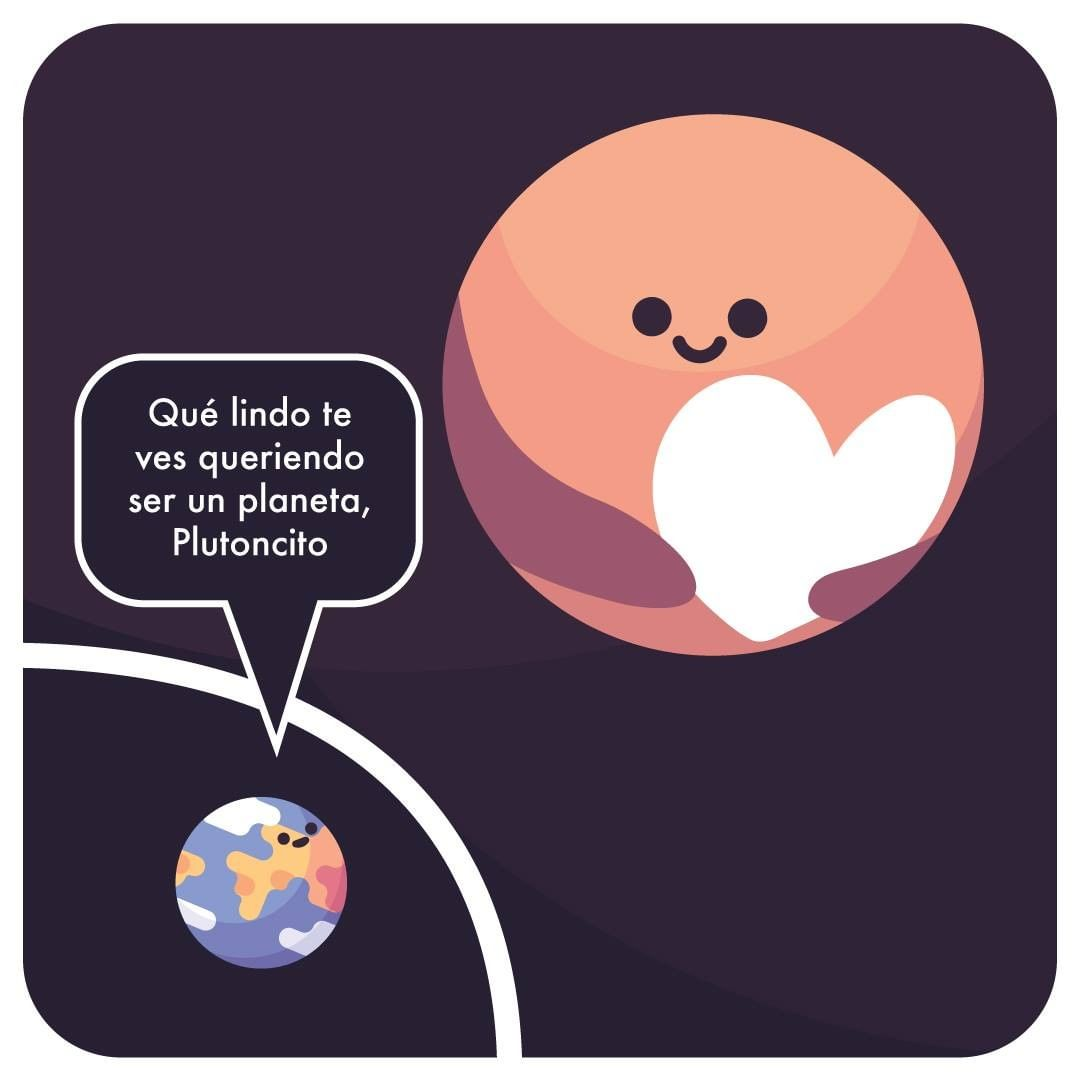
\includegraphics[width=\textwidth]{Pluton_1.jpg}
    %\caption*{Flower one.}
  \end{minipage}
  %\hfill
  \begin{minipage}[b]{0.4\textwidth}
    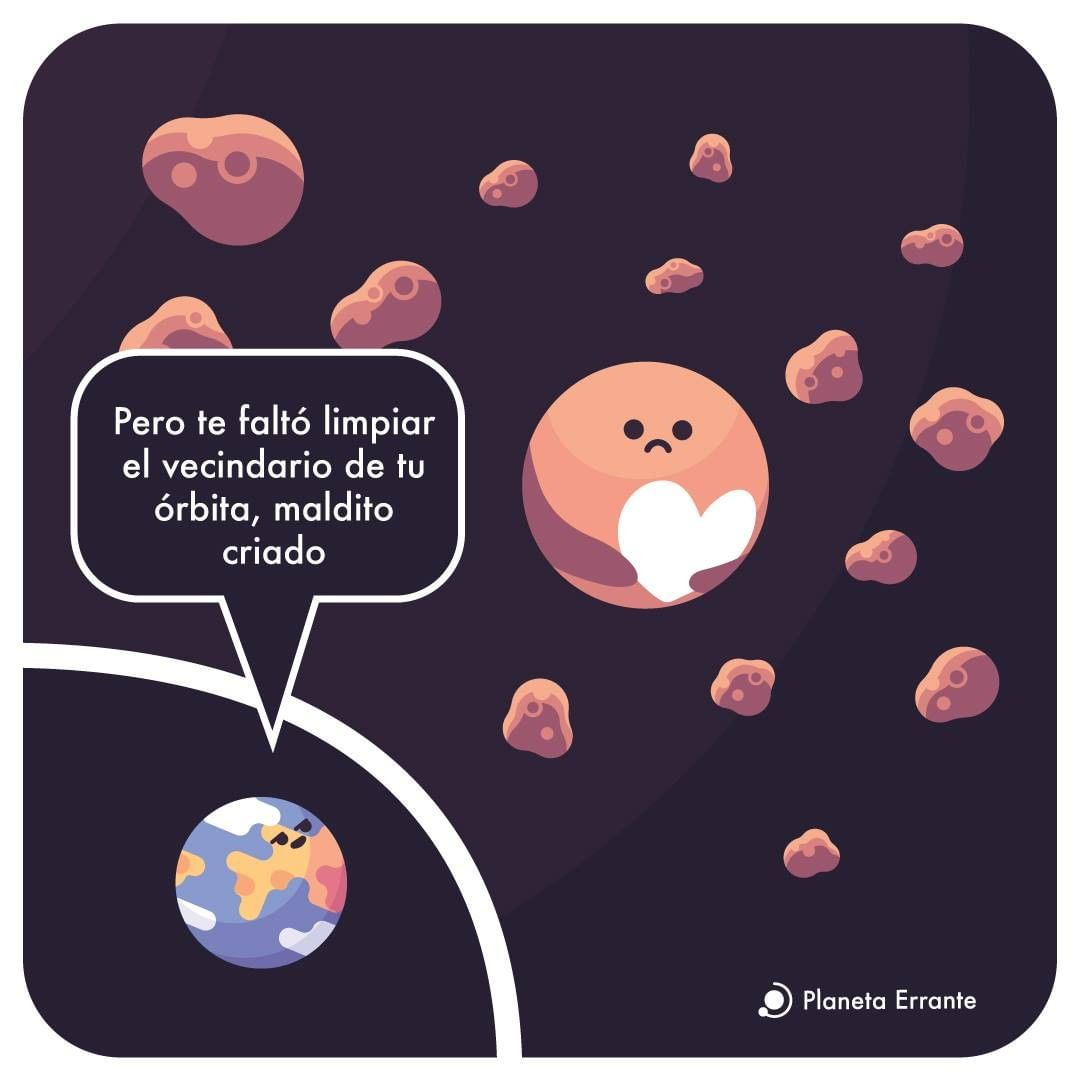
\includegraphics[width=\textwidth]{Pluton_2.jpg}
    %\caption*{Cr'editos: elplanetaerrante (Instagram)}
  \end{minipage}
  \captionsetup{justification=raggedleft,
singlelinecheck=false
}
\caption*{{\footnotesize Cr'editos: elplanetaerrante (Instagram)} }
\end{figure}

\vspace{3mm}

\textbf{Problema 2. Problemas generales}

\begin{enumerate}[a)]
\item \begin{myfont}Supongamos que observo dos estrellas y logro medir su color. Una de ellas resulta ser de color azul y la otra resulta ser de color rojo, ?`cu'al de las dos estrellas esperar'ia que fuera la m'as caliente y por qu'e?\end{myfont}


\emph{Soluci'on:}


Recordemos que la energ'ia ($E$) de un solo fot'on es proporcional a su frecuencia (la cual llamaremos con la letra griega $\nu$ [l'ease como ``n'u'']). Es decir,

\begin{equation}\label{en_prop}
E \propto \nu
\end{equation}

donde el s'imbolo ``$\propto$'' significa ``proporcional a''.

De manera que la proporci'on \eqref{en_prop} quiere decir que la energ'ia (de un fot'on) es proporcional a la frecuencia de 'este. Recordemos que el color de un fot'on nos dice algo sobre su frecuencia. Los colores \textcolor{blue}{azules} tienen una \emph{mayor frecuencia}; o, de igual manera, los colores m'as \textcolor{red}{rojizos} tienen una \emph{menor frecuencia}, todo esto en el espectro visible. Por lo tanto, en t'erminos energ'eticos, los fotones de color azul tienen una mayor frecuencia que los fotones de color rojo (\textcolor{blue}{Energ'ia color azul} > \ \textcolor{red}{Energ'ia color rojo}).

En espec'ifico, para que la proporci'on \eqref{en_prop} sea una igualdad debemos multiplicar por una constante. As'i, \emph{la energ'ia de un fot'on, en funci'on de su frecuencia, est'a dada por}:

\begin{equation} \label{energia_nu}
E = h \nu
\end{equation}

donde $h$ es la llamada ``constante de Planck'', la cual es una constante que aparece much'isimo en F'isica Cu'antica y la cual tiene un valor de $h = 6.62 \times 10^{-34} \ J \cdot s$.

De igual manera, podemos encontrar la energ'ia de un fot'on en funci'on de la longitud de onda ($\lambda$):

\begin{equation} \label{energia_nu}
E = h \cdot \frac{c}{\lambda}
\end{equation}

donde $c$ es la rapidez de la luz (un fot'on).

Ahora bien, mayores energ'ias (cin'eticas) se asocian a mayores temperaturas. Por lo tanto, es esperable que las estrellas m'as calientes sean m'as azules en comparaci'on a sus pares m'as rojizos. Por lo que, respondiendo a la pregunta del enunciado, esperar'iamos que la estrella azul sea m'as caliente que la roja.
\begin{myfont}\item ?`A qu'e distancia tendr'ia que estar una ampolleta de $100 \ W$ para que su flujo sea el mismo al flujo solar que recibe la Tierra? 

Para ello le puede servir de dato que la luminosidad del Sol es, aproximadamente, $L_\odot \approx 3.82 \times 10^{26} \ W \sim 4 \times 10^{26} \ W$.\end{myfont}

\emph{Soluci'on:}

Antes que todo, hay que preguntarnos ``¿qu'e es el flujo?''. Es normal que en el d'ia a d'ia escuchemos mucho esta palabra, y es bien utilizada en varios 'ambitos. La definici'on m'as general de flujo ser'ia la siguiente:

\begin{equation}
\text{Flujo} = \frac{\text{``Algo''}}{\text{'Area} \times \text{Tiempo}}
\end{equation}

Es decir, al medir el flujo estamos midiendo ``algo'' por unidad de 'area, por unidad de tiempo. ?`Por qu'e pongo un concepto tan abstracto como ``algo''? Porque, como dije, el concepto de flujo puede depender de qu'e es lo que queramos medir. Por ejemplo, si fu'esemos ingenieros especializados en transporte, ese ``algo'' nos interesar'ia que fueran autos o personas; si fu'esemos meteor'ologos nos interesar'ia que ese ``algo'' sea la cantidad de lluvia para as'i saber el monto ca'ido en una cierta 'area en un cierto tiempo; si fu'esemos ge'ografos nos interesar'ia que ese ``algo'' sea la cantidad de agua que pasa a trav'es de un cierto r'io y as'i. En astronom'ia, ese ``algo'' que nos interesa es la energ'ia. Por lo tanto, en astronom'ia, el flujo es:

\begin{equation} \label{flujo}
\text{Flujo} = \frac{\text{Energ'ia}}{\text{'Area} \times \text{Tiempo}}
\end{equation}

En astronom'ia adem'as est'a el concepto de luminosidad, el cual no es m'as que la potencia que emite una estrella en todas las direcciones. Recordemos que, desde la perspectiva f'isica, la potencia es la cantidad de trabajo que se realiza por unidad de tiempo, por lo que la luminosidad no es m'as que la energ'ia que emite una estrella por unidad de tiempo en todas las direcciones. En el Sistema Internacional (S.I.) la potencia se mide en watts y el trabajo en joules; o, en español'isimo t'io, en vatios y julios, respectivamente. Donde un watt es $1 \ \text{W} = 1 \ \frac{\text{kg} \cdot \text{m}^2}{\text{s}^3}$ y un joule es $1 \ \text{J} = 1 \frac{\text{kg} \cdot \text{m}^2}{\text{s}^2}$.

En resumen, matem'aticamente la luminosidad es:

\begin{equation} \label{luminosidad}
\text{Luminosidad} = \frac{\text{Energ'ia}}{\text{Tiempo}}
\end{equation}

Al comparar las ecuaciones \eqref{flujo} y \eqref{luminosidad}, vemos que hay una relaci'on entre flujo y luminosidad:

\begin{equation}
\text{Flujo} = \frac{\text{Luminosidad}}{\text{'Area}}
\end{equation}

M'as espec'ificamente, para un cierto flujo dado ($F$) de un objeto que que est'a a una cierta distancia ($d$) y que tiene una luminosidad ($L$) esta relaci'on es:

\begin{equation} \label{flujo_eq}
F = \frac{L}{4 \pi d^2}
\end{equation}

El factor $4 \pi d^2$ en el denominador es el 'area de una esfera de radio $d$  y viene de asumir que la estrella, en este caso el Sol, emite hacia  todas las direcciones con la misma intensidad (lo que se conoce como ``isotr'opico'') e ilumina de manera radial alrededor de 'el. De manera que ilumina formando una esfera alrededor de 'el. Es por esto que decimos que el \emph{flujo disminuye con el cuadrado de la distancia}. Esta relaci'on sigue siendo totalmente v'alida al querer comparar el flujo entre dos puntos distintos. Por ejemplo, si mido el flujo en la Tierra y mido el flujo en un punto que est'a a $2 \ \text{AU}$, esperar'ia que el flujo en aquel punto sea 4 veces menor comparado al flujo medido en la Tierra.

\begin{figure}[!ht]
\begin{center}
\begin{tabular}{ll}
  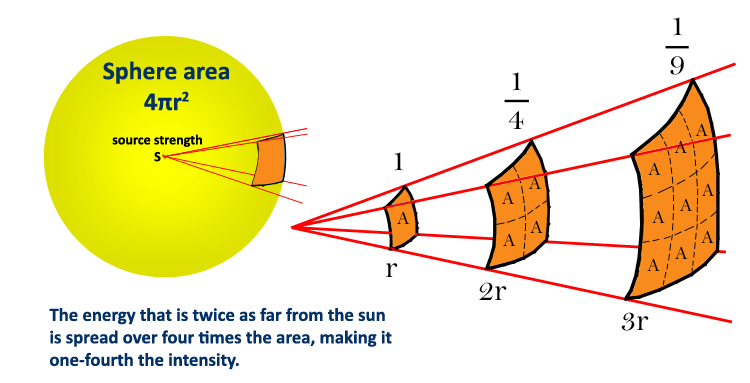
\includegraphics[width=0.6\textwidth]{solar.png} 
\end{tabular}
\caption{{\small A medida que nos alejamos de la estrella (u otra fuente emitiendo) la energ'ia que 'esta irradia se va esparciendo en un 'area cada vez m'as grande. Por lo que el flujo que medimos decrece con el cuadrado de la distancia. En nuestro problema, y compar'andolo con la figura, nosotros estamos usando la letra $d$ en vez de $r$, pero ambas respresentan lo mismo: la distancia desde el punto que emite luz.}}\label{fujo_cuadrado}
\end{center} 
\end{figure}


Volviendo al problema original del enunciado, sabemos que la distancia entre la Tierra y el Sol es, en promedio, una unidad astron'omica; lo que matem'aticamente es $1 \ \text{AU} = 1.496 \times 10^{11} \ \text{m}$. Lo que son, aproximadamente, unos 150 millones de kil'ometros. De manera que, en este caso en espec'ifico, la distancia ser'a $d = 1 \ \text{AU} = 1.496 \times 10^{11} \ \text{m}$. 

De manera que reemplazamos por los valores de $d$ y $L = L_\odot$ hallados y los usamos en la ecuaci'on \eqref{flujo_eq}, dando as'i:

\begin{equation*}
F = \frac{L}{4 \pi d^2} = \frac{L_\odot}{4 \pi (1 \ \text{AU})^2} = \frac{3.82 \times 10^{26} \ \text{W}}{4 \pi \cdot (1.496 \times 10^{11} \ \text{m})^2}
\end{equation*}

Obteniendo:

\begin{equation}
F = 1365 \frac{\text{W}}{\text{m}^2}
\end{equation}

Este valor se conoce como el valor de ``radiaci'on solar'' (o ``solar irradiance'' en ingl'es) y es tomado, aproximadamente, como constante. A alguien le pudo haber quedado la duda de porqu'e pas'e el par'ametro de la distancia $d$ de unidades astron'omicas a metros. Y la respuesta es que, personalmente, me gusta trabajar todo en el S.I. (o el sistema cgs\footnote{Sistema de Cent'imetros-Gramos-Segundos} en ciertos casos espec'ificos). Si hubi'esemos utilizado $d = 1 \ \text{AU}$, el resultado del flujo nos hubiese dado en unidades de $\frac{\text{W}}{\text{AU}^2}$, lo cual no es intuitivo porque son unidades, literalmente, astron'omicamente distintas en escala. Es por ello que siempre traten de trabajar todo en el mismo sistema de unidades.

Recordemos que queremos saber a qu'e distancia el flujo de una ampolleta de $100 \ \text{W}$ ser'a igual a la radiaci'on solar que acabamos de encontrar. Es por ello que lo que queremos hallar es la inc'ognita $d$ en la ecuaci'on \eqref{flujo_eq}. Despejando $d$ de 'esta se obtiene:

\begin{equation}
d = \sqrt{\frac{L}{4 \pi F}}
\end{equation}

Queremos conocer la distancia, pero esta vez desde la ampolleta de $100 \ \text{W}$ y queremos que el flujo sea igual a la Radiaci'on Solar reci'en encontrada. De manera que tenemos, finalmente:

\begin{equation*}
d = \sqrt{\frac{L}{4 \pi F}} = \sqrt{\frac{100 \ \text{W}}{4 \pi \cdot  1365 \ \text{W} \cdot \text{m}^{-2}}} = 7.63 \times 10^{-2} \ \text{m} = 7.63 \ \text{cm}
\end{equation*}

Es decir, cuando medimos el flujo a unos 7 cent'imetros y medio de distancia de una ampolleta de $100 \  \text{W}$, el flujo medido es casi igual al flujo que nos llega desde el Sol aqu'i en la Tierra (conocido como Radiaci'on Solar).

\begin{myfont} \item El Hubble Space Telescope (HST) est'a a una distancia de $\sim 610$ km sobre la superficie de la Tierra, ubicada en una 'orbita aproximadamente circular alrededor de 'esta. \end{myfont}




\begin{enumerate}[i)]
\begin{myfont}
\item Estime su per'iodo orbital.
\end{myfont}

\emph{Soluci'on:}

Siempre que les pregunten por per'iodos o distancias orbitales recuerden la Tercera Ley de Kepler, la cual es:

\begin{equation} \label{3era_ley_kepler_1}
\frac{P^2}{a^3} = \frac{4 \pi^2}{G (m_1 + m_2)} 
\end{equation}

donde $P$ es el per'iodo orbital (el tiempo que se demora en dar una vuelta el objeto que orbita), $a$ es la distancia promedio entre el objeto que orbita y el objeto m'as masivo, $G$ es la constante de gravitaci'on universal ($G = 6.67 \times 10^{-11} \ \text{N}\cdot \text{m}^2 \cdot \text{kg}^{-2} = 6.67 \times 10^{-11} \ \text{m}^3 \cdot \text{kg}^{-1} \cdot \text{s}^{-2}$); y $m_1$ y $m_2$ son las masas de los dos cuerpos interaccionando gravitacionalmente. Notemos que si $m_1 \gg m_2$ (l'ease el s'imbolo ``$\gg$'' como ``mucho mayor que'' o ``mucho m'as grande que'') eso quiere decir que la ecuaci'on \eqref{3era_ley_kepler_1} es casi igual a:

\begin{equation} \label{3era_ley_kepler_2}
\frac{P^2}{a^3} \approx \frac{4 \pi^2}{G \cdot m_1}, \ \ \ \ \ \ \ \ \text{si} \ m_1 \gg m_2
\end{equation}

Es decir, asumimos que $m_1 + m_2 \approx m_1$, si y s'olo si $m_1 \gg m_2$.

Muchas veces se ve esta ecuaci'on como:

\begin{equation*}
\frac{P^2}{a^3} = \text{Constante}
\end{equation*}

Y ello no est'a del todo mal. Si comparamos la Tercera Ley de Kepler para los planetas del Sistema Solar, $m_1$ siempre ser'a la masa del Sol y $m_2$ ser'a la masa del planeta. Como la masa del Sol, $m_1$, es mucho m'as grande que la masa de cualquier planeta $m_2$, sin importar qu'e planeta usemos el resultado a la derecha de la ecuaci'on \eqref{3era_ley_kepler_1} ser'a pr'acticamente siempre el mismo, es por ello que este valor se considera ``constante'' aunque realmente no lo sea.


Si le cuesta verlo, y si tiene tiempo, trate de calcular la parte derecha de la ecuaci'on \eqref{3era_ley_kepler_1} utilizando como $m_1$ la masa del Sol ($m_\odot \approx 1.98 \times 10^{30} \ \text{kg}$) y como $m_2$ cualquiera de las masas de los planetas dados en el Cuadro/Tabla \ref{tabla_planetas}. Ver'a que el resultado de $\frac{4 \pi^2}{G (m_1 + m_2)}$ es pr'acticamente el mismo sin importar qu'e masa planetaria utilice y es, por tanto, ``constante''.

?`Cu'ando este valor no es constante y debemos tener cuidado c'omo aplicarlo? Un ejemplo en concreto puede ser en los sistemas de estrellas binarias. Las estrellas binarias es un sistema estelar de dos estrellas que orbitan mutuamente entre s'i alrededor de un centro de masas. Como en este caso no se tiene que $m_1 \gg m_2$, entonces no se puede asumir un valor constante y por lo tanto, si bien s'i se puede utilizar Kepler para calcular su masa, hay que ser m'as cuidadosos.

\vspace{3mm}

Volviendo con el enunciado, queremos conocer el per'iodo orbital y por lo tanto debemos aplicar la Tercera Ley de Kepler (ecuaci'on \eqref{3era_ley_kepler_1}, o ecuaci'on \eqref{3era_ley_kepler_2} si la masa del cuerpo m'as masivo es mucho m'as grande que la del cuerpo orbitando [condici'on que s'i se cumple en este caso/ejercicio]). 

Nos dicen la distancia que hay entre el HST y la \emph{superficie} de la Tierra. Pero ojo, como dije es la distancia/altura a la \emph{superficie} de la Tierra, la cual llamaremos $h	$. Y para Kepler debemos utilizar la distancia al centro de masa, el cual asumimos que se encuentra exactamente al centro de la Tierra, a un radio terrestre o $R_\oplus = 6371 \ \text{km} = 6.37 \times 10^6 \ \text{m}$. Por lo tanto, la distancia entre el HST y el centro de masas del cual orbita est'a dado por:

\begin{equation*}
\text{Distancia al centro de masas} = (\text{Radio de la Tierra}) + (\text{Altura del HST a la superficie de la Tierra})
\end{equation*}

O matem'aticamente esto es igual a:

\begin{equation*}
a = R_\oplus + h = (6.37 \times 10^6 \ \text{m}) + (610 \times 10^3 \ \text{m}) = 6.99 \times 10^6 \ \text{m}
\end{equation*} 

Por otro lado, utilizando la masa de la Tierra como $m_1 = m_\oplus = 5.97 \times 10^{24} \ \text{kg}$ calculamos el lado derecho de la ecuaci'on \eqref{3era_ley_kepler_2} (ya que el HST debe tener una masa despreciable al lado del total de la masa de la Tierra), obteniendo:

\begin{equation} \label{cte_kepler_tierra}
\frac{4 \pi^2}{G \cdot m_1} = \frac{4 \pi^2}{(6.67 \times 10^{-11} \ \text{m}^3 \cdot \text{kg}^{-1} \cdot \text{s}^{-2}) \times (5.97 \times 10^{24} \ \text{kg})} = 9.91 \times 10^{-14} \ \text{s}^2 \cdot \text{m}^{-3} 
\end{equation}

Despejando el per'iodo orbital $P$ de la ecuaci'on \eqref{3era_ley_kepler_2} llegamos a:

\begin{equation} \label{periodo_kepler}
P = \sqrt{\frac{4 \pi^2}{G \cdot m_1} a^3}
\end{equation}

Y reemplazando por lo que acabamos de obtener en \eqref{cte_kepler_tierra} y  el valor de $a$ encontrado, tenemos que la ecuaci'on \eqref{periodo_kepler} da:

\begin{equation}
P = \sqrt{(9.91 \times 10^{-14} \ \text{s}^2 \cdot \text{m}^{-3}) \times (6.99 \times 10^6 \ \text{m})^3} = 5820 \ \text{s} \approx 97 \ \text{min}
\end{equation}

Es decir, el HST da una vuelta a la Tierra aproximadamente cada una hora y media.

\begin{myfont}
\item Los sat'elites de comunicaci'on y de monitoreos del clima usualmente est'an ubicados en lo que se conoce como 'orbitas de estacionamiento ``geos'incronas'' sobre la Tierra. La gracia de estas 'orbitas es que los sat'elites permanecen fijos sobre un punto espec'ifico sobre la Tierra. ?`A qu'e altitud deben estar localizados estos sat'elites?\end{myfont}

\emph{Soluci'on:}

Lo que requerimos esta vez es que el per'iodo orbital de los sat'elites sea igual al per'iodo de rotaci'on de la Tierra (de un d'ia sideral, 23h 56 min $\approx 23.93 \ \text{h}$).

Pasando la duraci'on del d'ia sideral a segundos obtenemos que 'este es, aproximadamente:

\begin{equation*}
P = 8.61 \times 10^4 \ \text{s}
\end{equation*}

(Si toma el per'iodo para un d'ia solar, asumir'a $P = 8.64 \times 10^4 \ \text{s}$ y el resultado ser'a levemente distinto, pero no radicalmente distinto)

De la ecuaci'on \eqref{3era_ley_kepler_2} podemos despejar $a$, obteniendo:

\begin{equation} \label{distancia_kepler}
a = \sqrt[3]{\frac{G \cdot m_1}{4 \pi^2} P^2}
\end{equation}

Podemos ``reciclar'' el resultado obtenido en la ecuaci'on \eqref{cte_kepler_tierra} y utilizarlo en la ecuaci'on \eqref{distancia_kepler} (pues es el mismo valor, pero elevado a $-1$), dando as'i:

\begin{equation*}
a = \sqrt[3]{\big( 9.91 \times 10^{-14} \ \text{s}^2 \cdot \text{m}^{-3} \big) ^{-1} \times (8.61 \times 10^4 \ \text{s})^2} = 4.22 \times 10^{7} \ \text{m}
\end{equation*}

Recordemos que $a$ es la distancia del HST al centro de masa, no es la altura desde la superficie. La altura $h$ viene dada simplemente por la diferencia entre el valor encontrado para $a$ y el radio de la Tierra (ya que, recordemos, $a = R_\oplus + h$):

\begin{equation}
h = a - R_\oplus
\end{equation}

As'i tenemos que:

\begin{equation*}
h = (4.22 \times 10^{7} - 6.37 \times 10^6) \ \text{m} = 3.58 \times 10^7 \ \text{m} = 5.6 \ R_\oplus.
\end{equation*}

Por lo que los sat'elites en 'orbitas geos'incronas est'an a, aproximadamente, unos 36 mil kil'ometros de altura.

\begin{myfont}
\item ?`Es posible que un sat'elite en una 'orbita geos'incrona permanezca ``estacionado'' sobre cualquier punto sobre la Tierra? ?`Por qu'e o por qué no?\end{myfont}

\emph{Soluci'on:}

Para que un sat'elite est'e ``estacionado'' debe estar sobre el Ecuador y orbitando en la misma direcci'on en la que la Tierra rota. Esto ya que el centro de la 'orbita del sat'elite es el centro de masa de la Tierra-sat'elite (que es prácticamente igual al centro de la Tierra).
\end{enumerate}

%\item Las estrellas circumpolares son estrellas que nunca se ponen bajo el horizonte para el observador local; o estrellas que nunca son visibles sobre el horizonte (nunca salen). 

%\begin{enumerate}[i)]
%\item Calcule el rango de declinaciones para estos dos grupos de estrellas (que se ven y no se ven) para un observador a una latitud L.

%\item ?`A qu'e latitud(es) en la Tierra el Sol nunca se podr'a cuando sea el solsticio de verano (en el hemisferio norte)?

%\item Basado en los dos sub-problemas anteriores, ?`existe alguna latitud en la Tierra donde el Sol nunca se pondr'a cuando sea el equinnocio vernal? De ser as'i, ?`d'onde?
%\end{enumerate} 
\vspace{3mm}

\begin{myfont}
\item Si nos encontrásemos en la ciudad de Lima (Perú), la cual tiene una latitud de $12^{\circ} S$ (o, equivalentemente, latitud de $-12^{\circ}$):\end{myfont} 

\begin{enumerate} [i)]

\begin{myfont}
\item ?`Cu'ales son las declinaciones (DEC) que se pueden ver en dicha ciudad?
\end{myfont}

\emph{Soluci'on:}

Observemos la Figura \ref{observable}. Las estrellas que uno puede observar desde una latitud $x^\circ$ est'an altamente restringidas por esta misma. Ya que, asumimos, para una latitud $x^\circ$ s'olo podemos observar en $90$ grados hacia el Norte y en $90$ grados hacia el Sur, \emph{todo esto desde su cenit} (sobre su cabeza). ?`Por qu'e $\pm 90^\circ$? Porque es la cantidad de grados que hay desde el cenit de uno hasta el horizonte. Obviamente esto podr'ia verse limitado por monta'nas u otros impedimentos, pero en principio/teor'ia uno deber'ia poder ver todas las estrellas desde el horizonte.

\begin{figure}[!ht]
\begin{center}
\begin{tabular}{ll}
  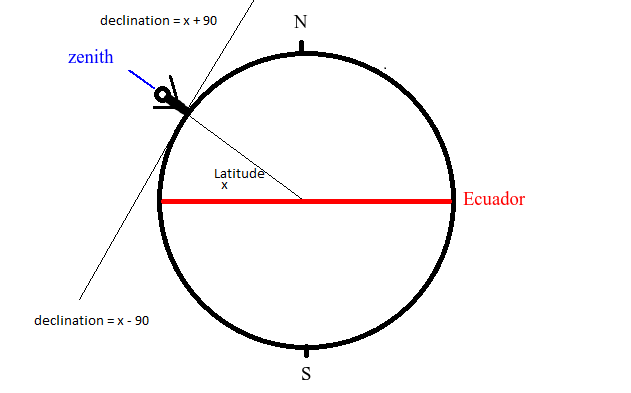
\includegraphics[width=0.6\textwidth]{observable.png} 
\end{tabular}
\caption{{\small Rango de declinaciones observables desde una latitud de $x^\circ$. Notemos que la persona, la cual se encuentra localizada en una latitud $x^\circ$, puede observar estrellas que est'an 90 grados hacia el Norte ($+90^\circ$) y estrellas que est'an 90 grados hacia el Sur ($-90^\circ$), \emph{todo esto desde su cenit} (sobre su cabeza) hacia el horizonte.}}\label{observable}
\end{center} 
\end{figure}

El rango en el cual se ve la estrella, matem'aticamente, podr'iamos definirlo como sigue:

\[ N(x) < \begin{cases} 
      (x+90)^\circ & , \ \text{si} \  (x+90)^\circ < 90^\circ \\
      90^\circ & , \ \text{si} \  (x+90)^\circ > 90^\circ \\
   \end{cases}
\]

\[ S(x) > \begin{cases} 
      (x-90)^\circ & , \ \text{si} \  (x-90)^\circ > -90^\circ \\
      -90^\circ & , \ \text{si} \  (x-90)^\circ < -90^\circ \\
   \end{cases}
\]

Y el rango en el cual se ver'a la estrella desde una latitud $x^\circ$ simplemente viene de intersectar ambos resultados, es decir,

\begin{equation}
D(x) = N(x) \cup S(x)
\end{equation}


S'e que puede parecer enredado (y lo es), pero sin tantas ecuaciones pi'ensenlo as'i:

Para una estrella de latitud $x^\circ$ hagan lo siguiente:

\begin{enumerate} [1)]
\item S'umenle $+90^\circ$ a la latitud $x^\circ$ donde se encuentran o desean conocer. Si el resultado es menor a $+90^\circ$, qu'edense con ese valor y an'otenlo. Ejemplo, si estamos en una latitud de 33 grados Sur, o $-33^\circ$, y le sumamos $+90^\circ$  el resultado es $+57^\circ$. Como ese valor es menor a $+90^\circ$ lo conservamos.

\item Si al sumar $+90^\circ$ a la latitud $x^\circ$ esta nos da m'as de $+90^\circ$, entonces elegimos el valor como $+90^\circ$. Por ejemplo, si estamos en una latitud de $+56^\circ$ y le sumamos $+90^\circ$ eso nos da $+146^\circ$. Como claramente eso es mayor a $+90^\circ$, entonces tomamos como ``cota superior'' un valor de $+90^\circ$ (ya que las declinaciones no llegan m'as allá de $\pm 90^\circ$).

\item S'umenle $-90^\circ$ a la latitud $x^\circ$ donde se encuentran o desean conocer. Si el resultado es mayor a $-90^\circ$, qu'edense con ese valor y an'otenlo. Ejemplo, si estamos en una latitud de 40 grados Norte, o $+40^\circ$, y le sumamos $-90^\circ$  el resultado es $-50^\circ$. Como ese valor es mayor a $-90^\circ$ lo conservamos.

\item Si al sumar $-90^\circ$ a la latitud $x^\circ$ esta nos da menos de $-90^\circ$, entonces elegimos el valor como $-90^\circ$. Por ejemplo, si estamos en una latitud de $-50^\circ$ y le sumamos $-90^\circ$ eso nos da $-140^\circ$. Como claramente eso es menor a $-90^\circ$, entonces tomamos como ``cota inferior'' un valor de $-90^\circ$.

\item Una vez hayamos obtenido los valores despu'es de haber sumado/restado $\pm 90^\circ$, simplemente hacemos una intersecci'on de los valores obtenidos y nos quedamos con ese rango. Por ejemplo, si al sumar $+90^\circ$ obtuve un valor de $+120$, ello quiere decir que asumimos un valor de $+90^\circ$ (pues $120^\circ > 90^\circ$). Y si al restar $90^\circ$ obtuvimos un valor de $-60^\circ$ nos quedamos con ese valor. Finalmente tomamos la intersecci'on entre los resultados de haber sumado/restado $\pm 90^\circ$, que en este ejemplo nos dar'ia un intervalo de $[-60^\circ,+90^\circ]$.
\end{enumerate}

\vspace{3mm}

Volviendo al problema original, deseamos conocer las declinaciones de las estrellas que se pueden ver desde Lima, Per'u; la cual tiene una latitud de 12 grados Sur, o equivalentemente, $-12^\circ$ (recuerden que latitudes hacia el hemisferio Norte son positivas y hacia el hemisferio Sur son negativas).

Al sumar $+90^\circ$ tenemos que esto es:

\begin{equation*}
-12^\circ+90^\circ = +78^\circ < 90^\circ
\end{equation*} Como $+78^\circ$ es menor a $+90^\circ$ todo est'a bien y conservamos este valor. 

Ahora sumamos $-90^\circ$. Esto nos da 

\begin{equation*}
-12^\circ-90^\circ = -102^\circ < -90^\circ \ \ \ \ \ \ \ \  \Rightarrow -90^\circ
\end{equation*} 

Como $-102^\circ$ es menor que $-90^\circ$, y eso no es posible, entonces asumimos un valor de $-90^\circ$ como cota inferior.

La intersecci'on de ambos valores hallados es entonces: $[-90^\circ, +78^\circ]$. 

\vspace{3mm}

Por lo que, desde Lima, Per'u, podemos ver en alguna 'epoca del a'no estrellas cuyo rango de declinaciones est'en entre $-90^\circ$ y $+78^\circ$.

\begin{myfont}
\item ?`Cu'al es la m'axima altura sobre el horizonte que puede alcanzar una estrella cuyas coordenadas ser'an $RA = 3^h : 00^m : 00^s$ y $DEC = +20^{\circ}$?
\end{myfont}

\emph{Soluci'on:}

Para entender bien este ejercicio hay que observar la Figura \ref{cielo}. Resalto y advierto que los 'angulos no est'an a escala en este dibujo, pero sirven para tener una noci'on de este ejercicio.

\newpage

\begin{figure}[!ht]
\begin{center}
\begin{tabular}{ll}
  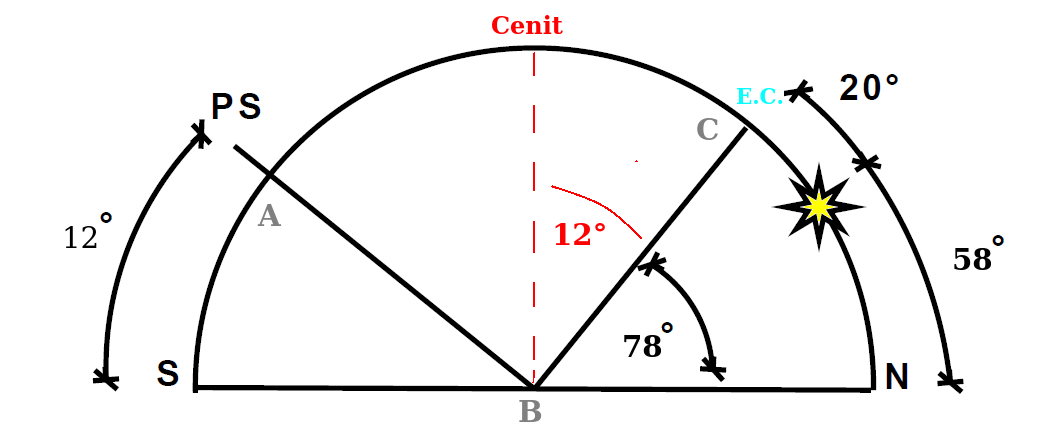
\includegraphics[width=0.8\textwidth]{cielo.png} 
\end{tabular}
\caption{{\small Alturas de una estrella sobre el horizonte. Los 'angulos no est'an a escala. Nótese c'omo la latitud define pr'acticamente todos los par'ametros: la altura del Polo Sur Celeste sobre el horizonte y la altura del Ecuador Celeste sobre el horizonte.}}\label{cielo}
\end{center} 
\end{figure}


Si tenemos una latitud de $+12^\circ$, ello quiere decir que si miramos hacia el sur (punto S en el dibujo) y luego empezamos a subir la mirada desde el horizonte hacia el cenit, el Polo Sur celeste estar'a $12^\circ$ sobre el horizonte. Una manera an'aloga de verlo es que, si empezamos a bajar la mirada desde el cenit hacia el horizonte, mirando hacia el norte, entonces all'i se encontrar'a el Ecuador Celeste (o el plano ecuatorial). Esto es porque la diferencia entre el Polo Sur celeste y el Ecuador celeste son $90^\circ$. Por lo que si el punto \textcolor{Gray}{A} en la Figura era el Polo Sur, entonces al sumarle un 'angulo recto ($\angle ABC$) obtendremos el Ecuador Celeste (punto \textcolor{Gray}{C} en la figura, que est'a en color \textcolor{Turquoise}{turquesa} tambi'en). 

Adem'as, si observa la Figura \ref{ra_y_dec} un par de p'aginas m'as adelante, ver'a que la declinaci'on es un 'angulo que se mide desde el Ecuador Celeste. Es positivo si lo medimos hacia el Norte y negativo si lo medimos hacia el Sur.

$\bullet$ Para el Hemisferio Sur:

Entonces, de la Figura \ref{cielo}, vemos que la altura de un objeto sobre el horizonte -mirando hacia el norte- estar'a dada por:

\begin{equation} \label{altura}
H = 90^\circ + \text{LAT} - \text{DEC}
\end{equation} 

donde $\text{LAT}$ es la latitud -la cual ser'a positiva para el hemisferio Norte, y negativa para latitudes del hemisferio Sur- (un s'imbolo alternativo para la latitud es usando la letra griega $\Phi$ [l'ease como ``fi'']) y $\text{DEC}$ (o $\delta$) es la declinaci'on del objeto que queremos observar.


Por lo que es com'un encontrar la ecuaci'on \eqref{altura} como:

\begin{equation} \label{altura_2}
H = 90^\circ + \Phi - \delta
\end{equation}

Las ecuaciones \eqref{altura} y \eqref{altura_2} son completamente iguales, s'olo usamos distinta notaci'on.  \emph{Esta ecuaci'on que hemos encontrado es v'alida para el hemisferio Sur y si la altura encontrada es menor o igual a} $90^\circ$.

Si la altura que nos resulta de aplicar la ecuaci'on \eqref{altura_2} a una estrella super'ase los $90^\circ$ entonces de la Figura \ref{altura} podemos ver que se puede utilizar la relaci'on:

\begin{equation} \label{altura_3}
H = 180^\circ - (90^\circ + \Phi - \delta)
\end{equation}

Lo cual nos dar'a la altura de la estrella sobre el horizonte mirando hacia el Sur.

\newpage

$\bullet$ Para el Hemisferio Norte:

Observemos la Figura \ref{cielo_2}, la cual es el caso para un observador situado en el hemisferio Norte:

\begin{figure}[!ht]
\begin{center}
\begin{tabular}{ll}
  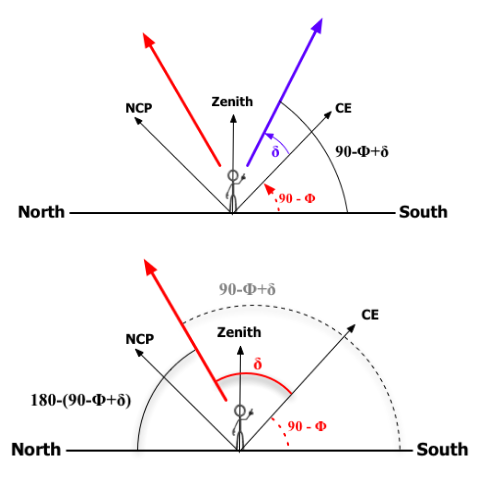
\includegraphics[width=0.5\textwidth]{altura_2.png} 
\end{tabular}
\caption{{\small Alturas de una estrella sobre el horizonte para un observador en el hemisferio Norte.}}\label{cielo_2}
\end{center} 
\end{figure}

Vemos que podemos encontrar una relaci'on similar a la hallada en el hemisferio Sur, pero esta vez la altura mirando hacia el Sur estar'a dada por:

\begin{equation} \label{altura_norte}
H = 90^\circ - \Phi + \delta
\end{equation}

Y si la altura que nos resulta de aplicar esta ecuaci'on a una estrella es mayor de $90^\circ$, entonces -y basados en el dibujo- podemos decir que la estrella tendr'a una altura:

\begin{equation} \label{altura_norte_2}
H = 180^\circ - (90^\circ - \Phi + \delta)
\end{equation}

lo cual nos dar'a la altura de la estrella sobre el horizonte mirando hacia el Norte.

\vspace{3mm}


Una vez explicado esto volvamos al ejercicio original: una estrella con coordenadas $RA = \alpha = 03^h$ y $\delta = +20^\circ$.

Como estamos en el hemisferio Sur podemos observar la Figura \ref{cielo}. De ella hemos -justificadamente- derivado la ecuaci'on \eqref{altura_2}. Por lo que la altura ser'a simplemente aplicar:

\begin{equation*}
H = 90^\circ + \Phi - \delta
\end{equation*} 

Que reemplazando con los datos dados es:

\begin{equation*}
H = 90^\circ + (-12^\circ) - (+20^\circ) = 90^\circ - 12^\circ - 20^\circ = 58^\circ
\end{equation*}

De manera que la m'axima altura que alcanzar'a esta estrella, vista desde Lima, Per'u, ser'a de $58^\circ$ sobre el horizonte mirando hacia el Norte.

\newpage

\begin{myfont}
\item ?`Cu'al es la mejor fecha para ver dicha estrella?
\end{myfont}

\emph{Soluci'on:}

Aqu'i hay dos maneras de saber esto: la primera es ``memorizarse'' la Tabla/Cuadro \ref{fechas} (aunque no es necesario memorizarse todas, con saber una sola fecha y ascensi'on recta respectivos al mes que le sigue se le suman 2 horas a la ascensi'on recta y as'i; por lo que sabiendo una sola se puede deducir todo el resto).

Pero obviamente est'an en la universidad y, a diferencia del colegio/liceo, muchas cosas ya no aparecen por arte de magia y son verdad s'olo porque el profesor el ayudante las dice.

\vspace{3mm}

\begin{center}
\begin{tabularx}{\linewidth}{*{2}{C}} \toprule
D'ia & Ascensi'on recta ($\text{hora}$) \\\midrule
$21$ de Marzo   & $12:00:00$    \\ 
 $21$ de Abril & $14:00:00$  \\ 
 $21$ de Mayo & $16:00:00$  \\
 $21$ de Junio & $18:00:00$ \\
 $21$ de Julio & $20:00:00$ \\
 $21$ de Agosto & $22:00:00$ \\
 $21$ de Septiembre & $00:00:00$ \\
 $21$ de Octubre & $02:00:00$   \\
 $21$ de Noviembre & $04:00:00$  \\
 $21$ de Diciembre & $06:00:00$ \\
 $21$ de Enero& $08:00:00$\\
 $21$ de Febrero & $10:00:00$ \\\bottomrule
\hline
\end{tabularx}
\captionof{table}{Ascensi'on recta correspondiente (\textbf{a la medianoche}) seg'un los d'ias del a'no. Reitero (porque hay gente que se confunde) que esto es a la \textbf{medianoche}.} \label{fechas}
\end{center}

\vspace{3mm}

Recuerden que el 21 de Marzo es el punto que se conoce como Punto Aries, y es el ``punto de comienzo'' donde el Sol est'a en el origen tanto de las ascenciones rectas como de las declinaciones (es decir, el 21 de Marzo el Sol tiene coordenadas $RA = 0^h : 00^m : 00^s$ y $DEC = +00.00^{\circ}$). Piensen que, totalmente opuesto al Sol, est'an las estrellas cuyas ascenciones rectas son $+12$ h con respecto a 'este.

Para entenderlo mejor, observen la Figura \ref{ra_y_dec}. 

\begin{figure}[h!]
\centering
\begin{subfigure}{.5\textwidth}
  \centering
  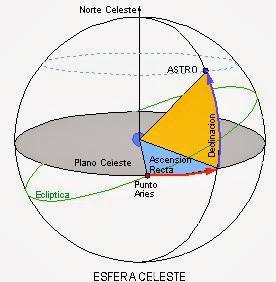
\includegraphics[width=.6\linewidth]{esfera.jpg}
  \caption{Esfera Celeste y sus elementos}
  \label{fig:sub1}
\end{subfigure}%
\begin{subfigure}{.5\textwidth}
  \centering
  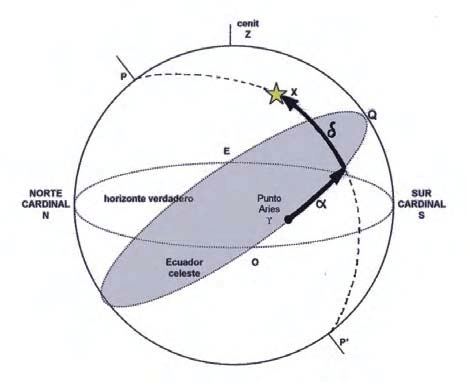
\includegraphics[width=.8\linewidth]{ra_y_dec.png}
  \caption{Ascensi'on recta y declinaci'on}
  \label{fig:sub2}
\end{subfigure}
\caption{Ascensi'on recta y declinaci'on}
\label{ra_y_dec}
\end{figure}

Poniendo especial 'enfasis en la Figura \ref{ra_y_dec} (izquierda), el \textcolor{Gray}{Ecuador Celeste} est'a en color \textcolor{Gray}{gris}, la \textcolor{NavyBlue}{Tierra} es la esfera \textcolor{NavyBlue} {azul} al centro, la \textcolor{Cyan}{Ascensi'on Recta} est'a en \textcolor{Cyan}{celeste}, la \textcolor{Dandelion}{Declinaci'on} en \textcolor{Dandelion}{naranjo} y la \textcolor{ForestGreen}{ecl'iptica} en \textcolor{ForestGreen}{verde}. El Sol estar'a en el \textcolor{Red}{Punto Aries} (punto-c'irculo \textcolor{Red}{rojo}). Imaginen que el Sol estar'a saliendo de la pantalla de su notebook/celular, en la Figura \ref{ra_y_dec}(a), cuando se encuentre en el Punto Aries; mientras que las estrellas que est'en al ``otro lado'' (las estrellas que estar'ian detr'as de la pantalla) estar'ian ubicadas en el lugar si sumamos 12 horas a la Ascensi'on Recta (es decir, dejamos avanzar la Ascensi'on Recta 12 horas [zona celeste en el dibujo]). Como el Sol se encuentra desde nuestro lado de la pantalla, pero las estrellas visibles est'an detr'as de la pantalla, ello quiere decir que las estrellas ``'optimas'' para ser vistas est'an totalmente opuestas a la posici'on del Sol; pues, al otro lado del mundo ser'a de noche.

Entonces lo que yo hago es ``deducir'' la Tabla/Cuadro \ref{fechas}, recordando que el Punto Aries (el origen de las coordenadas) es el 21 de Marzo. Como el 21 de Marzo el Sol tendr'a Ascensi'on Recta $RA =  0^h : 00^m : 00^s$, las estrellas tienen que estar -por lo que expliqu'e m'as arriba- en una Ascensi'on Recta de $+12$ horas con respecto al Sol. As'i, las estrellas el 21 de Marzo, a medianoche, tendr'an una Ascensi'on Recta de $RA = 12^h$. Cada mes que pasa va agregando 2 horas a la Ascensi'on Recta de las estrellas en la tabla (pues el Sol va avanzando, cada mes, 2 horas de Ascensi'on Recta); de manera que si el 21 de Marzo eran $RA = 12^h$, el 21 de Abril ser'an $RA = 14^h$, el 21 de Mayo ser'an $RA = 16^h$, el 21 de Junio ser'a $RA = 18^h$ y as'i...

De manera que esta tabla puede construirse justificadamente (m'as all'a de memorizarla). Para fines pr'acticos, memorizarla est'a bien, pero si quieren ir un poco m'as all'a entender de d'onde viene es bastante importante. 

Mirando la Tabla \ref{fechas} vemos que la Ascensi'on Recta de $03^h$ -que es la que nos han dado en el enunciado- cae, aproximadamente, entre el 21 de Octubre y el 21 de Noviembre. Por lo que asumimos que est'a ``a la mitad'' de estas dos fechas, es decir, el 5 de Noviembre. Por lo que la fecha en donde mejor se ver'a\footnote{Con ``mejor se ver'a'' me refiero a que su altura sobre el horizonte ser'a la m'axima posible, es decir, pasar'a lo m'as cerca del cenit posible.} esta estrella ser'a a principios de Noviembre.

\begin{myfont}
\item ?`Qu'e pasa si ahora observamos otro astro con la misma Ascensi'on Recta, pero con declinaci'on levemente diferente de $DEC = +5^{\circ}$? \end{myfont}

\emph{Soluci'on:}

Asumiendo que la declinaci'on cambia, pero la ascensi'on recta se mantiene igual, la nueva estrella tendr'a coordenadas $\alpha = 03^h; \delta = +5^\circ$. Asumiendo que seguimos observando esta estrella desde Lima, Per'u, si observamos la Figura \ref{cielo} lo 'unico que har'ia este cambio de declinaci'on es que el 'angulo que dice ``$20^\circ$'' en aquella figura, ahora ser'ian $5^\circ$. Por lo que la estrella tendr'ia una altura mayor respecto al horizonte.

Esto se reafirma si utilizamos la ecuaci'on \eqref{altura_2} encontrada:

\begin{equation*}
H = 90^\circ + \Phi - \delta
\end{equation*}

Lo que ser'ia:

\begin{equation*}
H = 90^\circ + (-12^\circ) - (+5^\circ) = 90^\circ - 12^\circ - 5^\circ = 73^\circ
\end{equation*}

Por lo que, respondiendo al enunciado, la nueva estrella ahora tendr'ia una altura de $73^\circ$; en comparaci'on de los $58^\circ$ sobre el horizonte de la estrella anterior. Como la ascensi'on recta de ambas es la misma, ambas se ver'an en la misma fecha del a'no.

\begin{myfont}
\item ?`Cu'al es entonces ``la mejor'' declinaci'on que puede tener una estrella para ser observada en las mejores condiciones posibles? Esto es, que pase justo a $90^{\circ}$ sobre el horizonte. \end{myfont}

\emph{Soluci'on:}

Basados en la Figuras \ref{cielo} y \ref{cielo_2}, una estrella pasa por nuestro cenit (justo encima de nuestra cabeza) cuando la declinaci'on de la estrella y la latitud son iguales. De esta manera, la estrella alcanzar'a una altura m'axima de $90^\circ$ sobre el horizonte. Al estar en el punto m'as alto posible, la luz de la estrella pasa por la menor cantidad de atm'osfera, lo que ocasiona que la luz se vea menos modificada por la atm'osfera terrestre. Este es el caso ``ideal'' de observaci'on para cualquier objeto.

Esto se reafirma con las ecuaciones -que hemos encontrado- \eqref{altura_2} y \eqref{altura_norte}, donde si asumimos $\Phi = \delta$ obtenemos para ambas:

\begin{itemize}

\item Para el hemisferio Sur:
\begin{equation*}
H = 90^\circ + \Phi - \delta = 90^\circ + \Phi - \Phi = 90^\circ
\end{equation*}

\item Para el hemisferio Norte:

\begin{equation*}
H = 90^\circ - \Phi + \delta = 90^\circ - \Phi + \Phi = 90^\circ
\end{equation*}

\end{itemize}

Por lo que, sin importar en qu'e hemisferio nos encontremos, si la latitud de un lugar es la misma con la declinaci'on de una estrella, la estrella pasar'a exactamente por el cenit de un observador ubicado en dicha latitud; esta es la condici'on ``ideal'' para observar una estrella. Ello quiere decir, por ejemplo, que si usted sale a su patio a mirar una estrella y esta puede verse casi sobre su cabeza, la declinaci'on de esa estrella es bastante similar a la latitud en la cual usted se encuentra. Por ejemplo, si en Santiago vemos una estrella que pasa casi por nuestro cenit, podemos decir que esa estrella tiene una declinaci'on de $-33^\circ$, ya que la latitud de Santiago es de $-33^\circ$.

De manera que la declinaci'on ($\delta$) nos dice dos cosas: i) ?`Se puede o no ver el objeto que deseamos? ii) Si se puede ver, ?`qu'e tan alto sobre el horizonte pasa aquel objeto? Por otro lado, la ascensi'on recta ($\alpha$) nos dice en qu'e momento del a'no es esa estrella visible y transitar'a por nuestro cielo observable.


\begin{myfont}
\item El centro gal'actico tiene coordenadas $RA = 17^h:45^m:40.04^s$ y $DEC = -29^{\circ} 00^{\prime} 28.1^{\prime \prime}$. ?`Qu'e puede decir sobre esto si lo relaciona con la posici'on de los telescopios gigantes que se encuentran en el Norte de Chile?
\end{myfont}

\emph{Soluci'on:}

La mayor'ia de los telescopios de Chile se encuentran, como todos sabemos, en el Norte de Chile. Estos observatorios est'an ubicados por la latitud $-26^\circ$ y alrededores. ?`Qu'e quiere decir esto? Que el centro de la V'ia L'actea pasa en el mes de Junio\footnote{Mire la Tabla \ref{fechas} si no sabe porqu'e es Junio.} casi en el cenit de aquellos lugares. Es por ello, por ejemplo, que hay un survey encargado de ``escanear'' el centro de la V'ia L'actea llamado VVV (The VISTA Variables in The Via Lactea) el cual est'a ubicado en el Observatorio Paranal, ubicado en el Norte de Chile en la latitud $-24^\circ36^\prime57^{\prime \prime}$. Ello quiere decir que la latitud de este telescopio es muy similar a la declinaci'on del centro de la V'ia L'actea. Lo que lo hace 'optimo para estudiarlo (adem'as de los limpios cielos, claro est'a). Un dato in'util-curioso extra es que el VVV observa el centro de la V'ia L'actea en luz infrarroja. Si observ'asemos el centro de la V'ia L'actea con luz visible no ver'iamos nada, ya que hay una gran cantidad de polvo que no nos permite observar directamente con luz visible. Pero este polvo se hace ``invisible'' si observamos con luz infrarroja, lifehacks que usan los astr'onomos.

\end{enumerate}
\end{enumerate}

\begin{figure}[!ht]
\begin{center}
\begin{tabular}{ll}
  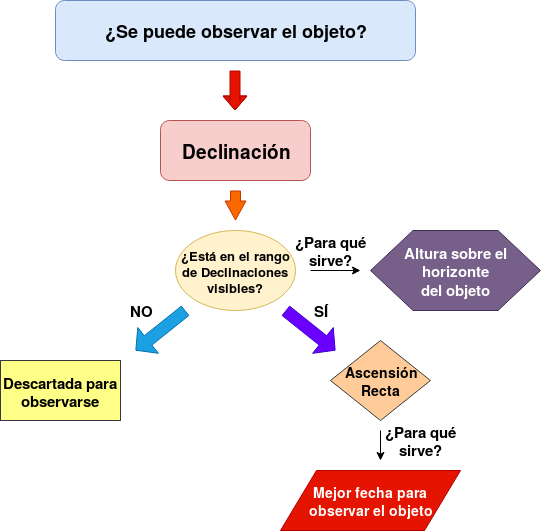
\includegraphics[width=0.55\textwidth]{diagrama.png} 
\end{tabular}
%\caption{{\small Alturas de una estrella sobre el horizonte para un observador en el hemisferio Norte.}}\label{cielo_2}
\end{center} 
\end{figure}



\end{document}